\section{Grundlegende Begriffe und Definitionen}

In diesem Kapitel sollen kurz die wichtigsten Begriffe für die softwaregestützten Analyse des Einflusses der zunehmenden Netzintegration von Elektrofahrzeugen auf die Verteilnetze definiert und erläutert werden.


\subsection{Stromnetz}

Das Stromnetz dient der Übertragung und Verteilung von elektrischer Energie. \cite{Paschotta2020}
Dabei lässt sich das Stromnetz in verschiedene Netzebenen aufteilen, welche jeweils typische Charakteristika aufweisen.
Innerhalb dieses Kapitels sollen diese kurz beschrieben und weitere wichtige Begriffe im Zusammenhang mit Stromnetzen erläutert werden.


\paragraph{Netzebenen:}

Das Stromnetz lässt sich grundsätzlich in Übertragungs- und Verteilnetze unterteilen.
Das Übertragungsnetz dient dem Transport von Strom über lange Strecken bei hohen Spannungen.
Ergänzend erfolgt in den Verteilnetzen die regionale Feinverteilung bei geringeren Spannungen. \cite{Agora2019}\medskip

Innerhalb der Verteilnetze wird zwischen drei Spannungsebenen unterschieden.
Hierzu zählen die \glspl{HS}-, \glspl{MS}- und \glspl{NS}-Ebene.
In \autoref{tab:Spannungsebenen} finden sich die üblichen Spannungen je Spannungsebene und die verbaute Stromkreislänge in Deutschland je Spannungsebene.
Innerhalb dieser Masterarbeit werden ausschließlich die Effekte auf die Verteilnetze auf der \glspl{MS}- und \glspl{NS}-Ebene untersucht.
Zusätzlich erfolgt eine Betrachtung der Effekte auf die Umspannebene der \gls{MS}-\gls{NS}-\glspl{USW}.

{
\renewcommand{\arraystretch}{1.2}% grßerer Zeilenabstand
\sisetup{range-phrase=~bis~}
\begin{table}[H]
	\begin{center}
		\caption{Übliche Spannung und Stromkreislänge der Spannungsebenen im deutschen Verteilnetz}
		\begin{tabu} to 0.65\textwidth {X[0.75] X[1, r] X[1, r]}
			\toprule
            Spannungsebene & Spannung               	& Stromkreislänge   \\\midrule
            Hochspannung   & \SIrange{60}{110}{\kv}     & \SI{95000}{\km}   \\
            Mittelspannung & \SIrange{6}{30}{\kv}  		& \SI{510000}{\km}  \\
            Niederspannung & \SI{230}{\V} 				& \SI{1100000}{\km} \\\bottomrule
            \multicolumn{3}{l}{Quellen: \cite{BDEW2016} und \cite{BMWiNetz}}
		\end{tabu}
		\label{tab:Spannungsebenen}
	\end{center}
	\vspace{-3mm}%Put here to reduce too much white space after your table
\end{table}
}


\paragraph{Netztopologie:}

\gls{NS}-Netze werden in dieser Arbeit als Strahlennetze ausgelegt.
Strahlennetze werden so genannt, weil die einzelnen Stränge der Netze strahlenförmig vom Ortsnetztransformator zu den Endverbrauchern verlaufen. \cite{Agora2019}
Vorteil dieser Form von Netzen ist die leichte Berechenbarkeit und die einfache Überwachung des Netzzustandes.
Jedoch führt bereits ein einziger Fehlerfall an einer Einspeisestelle eines Verbrauchers dazu, dass auch alle nachfolgenden Verbraucher vom Netz getrennt werden.
Auch nimmt der Spannungsabfall über die Länge der Leitung immer weiter zu, was zu einer geringeren Belastbarkeit am Ende der Leitung führt. \cite{WNG2020}\medskip

Im Gegensatz zu \gls{NS}-Netzen werden \gls{MS}-Netze als Ringnetze ausgelegt.
Ringnetze bieten den Vorteil, dass diese von zwei Seiten gespeist werden, wodurch ein Ringform entsteht.
Hierdurch können im Falle einer Störung weiterhin alle anderen Verbraucher versorgt werden.
Jedoch werden Ringnetze in der Praxis meist offen betrieben.
Dies bedeutet, dass sich etwa in der Mitte des Rings eine offene Trennstelle befindet.
Auf diese Weise können Ringnetze ebenso einfach überwacht werden wie Strahlennetze.
Im Fehlerfall wird so maximal ungefähr die Hälfte der Verbraucher vom Netz getrennt.
Durch das Schließen der Trennstelle können dann wieder alle Verbraucher, mit Ausnahme des Fehlerfalls, versorgt werden. \cite{WNG2020} \cite{Westermann2019}


\paragraph{Gleichzeitigkeit:}

Die Gleichzeitigkeit beschreibt den Anteil der momentan anfallenden elektrischen Leistung von der maximalen elektrischen Leistung im Netzgebiet. \cite{Agora2019} 
Im Rahmen dieser Masterarbeit beschreibt die Gleichzeitigeit in der Regel den Anteil der momentanen elektrischen Last von \glspl{EPKW} im Bezug auf die installierte Leistung von Ladepunkten in einem Netzgebiet.
Ausnahmen sind entsprechend gekennzeichnet.


\paragraph{Elektrische Flexibilität:}

Elektrische Flexibilität beschreibt die Fähigkeit des Stromsystems, trotz einer vorhergesehene oder unvorhergesehene Änderungen im Verbrauch oder der Erzeugung einen Ausgleich zwischen Angebot und Nachfrage aufrecht zu erhalten.
Dabei wird die Reaktion des Stromsystems durch ein externes Signal ausgelöst.
Bei dem externen Signal kann es sich beispielsweise um ein Preissignal, aber auch ein physikalisch messbares Signal, wie die Netzfrequenz, handeln. \medskip

Elektrische Flexibilität besitzt sowohl eine zeitliche als auch eine geografische Dimension.
Die zeitliche Dimension beschreibt die zeitliche Verschiebung von Last oder Erzeugung und reicht von einer sekündlichen bis zu einer saisonalen Verschiebung.
Unter der geografischen Dimension wird die gemeinsame Nutzung von räumlich verteilten Ressourcen verstanden.
Dabei reicht die räumliche Skala von lokalen Quartierslösungen bis zu internationalen Verbundnetzen. \cite{BNetzA2017} \cite{IEA2014}


\paragraph{Residuallast:}

Die Residuallast beschreibt die Differenz zwischen der benötigten Leistung und der erbrachten Leistung von nicht steuerbaren Kraftwerken innerhalb eines Betrachtungsgebietes.
Aufgrund des zunehmenden Anteils von nicht steuerbaren regenerativen Kraftwerken im Stromnetz und der fortschreitenden Sektorkopplung steigt zunehmend die Spreizung zwischen dem maximalen Wert und dem minimalen Wert der Residuallast.\medskip

% TODO: Eventuell Entwicklung drastellen

Positive Residuallast wird derzeit zu großen Teilen durch regelbare Kraftwerke gedeckt, während negative Residuallast durch die Abregelung von nicht steuerbaren Kraftwerken ausgeglichen wird.
Alternativ kann eine Glättung der Residuallast auch durch die Steuerung des Verbrauches erreicht werden, wodurch vor allem negative Residuallast ausgeglichen werden kann.
Aufgrund der hohen Ladeleistungen bieten \gls{EPKW} hierfür ein großes Potential. \cite{Paschotta2020a}


\paragraph{Netzprobleme:}

Probleme im Netz entstehen durch eine Überlastung von Betriebsmitteln im Stromnetz oder eine Verletzung des Spannungsbandes bei Endverbrauchern.
Bei der Ermittlung von Netzproblemen müssen grundlegend zwei Fälle unterschieden werden.
Im Lastfall überwiegt der Energiebedarf der Verbraucher gegenüber der Energiebereitstellung der Erzeugerkapazitäten im Netzgebiet.
Das Netz muss in diesem Fall in der Lage sein, bereitgestellte Energie aus den überlagerten Netzebenen an die Verbraucher weiterzuleiten.
Im Rückspeisefall überwiegt hingegen die Energiebereitstellung der Erzeugerkapazitäten gegenüber dem Energiebedarf der Verbraucher und der erzeugte Strom muss an die überlagerten Netzebenen weitergeleitet werden können. \cite{Agora2019}
Für die Betriebsmittel gelten die in \autoref{tab:Belastungsfaktoren} und \autoref{tab:Spannungsband} zulässigen Belastungsfaktoren und Spannungsabweichungen, welche aus \cite{Mueller2019a} entnommen wurden und auf der Verteilnetzstudie für das Land Baden-Württemberg \cite{Rehtanz2017} basieren.


\subparagraph{Verletzungen der thermische Betriebsmittelbelastungen} treten auf, wenn die physikalischen Grenzen von Betriebsmitteln bezüglich ihrer Scheinleistungsbelastbarkeit übertreten werden.
Der Belastungsfaktor eines Betriebsmittels gibt an, inwieweit ein Betriebsmittel mit Nennscheinleistung belastet werden kann.
Dabei spiegeln die Belastungsfaktoren wieder, dass für Verbraucher, welche im \gls{MS}-Netz angeschlossen sind, das (n-1)-Kriterium  gilt.
Dies gilt in der Regel jedoch nicht für Verbraucher im \gls{NS}-Netz und Erzeugerkapazitäten, welche im \gls{MS}- oder \gls{NS}-Netz angeschlossen sind.
Die Belastungsfaktoren der einzelnen Betriebsmittel sind in \autoref{tab:Belastungsfaktoren} zusammengefasst. \cite{Schachler} \cite{Rehtanz2017}


{
\renewcommand{\arraystretch}{1.2}% grßerer Zeilenabstand
\sisetup{range-phrase=~bis~}
\begin{table}[H]
	\begin{center}
		\caption{Zulässige Belastungsfaktoren der Betriebsmittel in der MS- und NS-Ebene}
		\begin{tabu} to 0.6\textwidth {X[1.6] X[0.8, r] X[1, r]}
			\toprule
			Betriebsmittel      & Lastfall           & Rückspeisefall     \\ \midrule
			MS Kabel            & \SI{50}{\percent}  & \SI{100}{\percent} \\
			NS Kabel            & \SI{100}{\percent} & \SI{100}{\percent} \\
			HS-MS-Transformator & \SI{50}{\percent}  & \SI{100}{\percent} \\
			MS-NS-Transformator & \SI{100}{\percent} & \SI{100}{\percent} \\ \bottomrule
            \multicolumn{3}{l}{Quelle: \cite{Rehtanz2017}}
		\end{tabu}
		\label{tab:Belastungsfaktoren}
	\end{center}
	\vspace{-3mm}%Put here to reduce too much white space after your table
\end{table}
}


\subparagraph{Verletzungen des Spannungsbandes} treten bei einer starken Abweichung der Spannung am Betriebsmittel von der Nennspannung auf.
Die zulässigen Spannungsabweichungen liegen für Endkunden in der \gls{NS}-Ebene bei \SI{\pm 10}{\percent}.
Dieses Spannungsband wird nach \autoref{tab:Spannungsband} auf die \gls{MS}, \gls{MS}-\gls{NS}- und \gls{NS}-Ebene aufgeteilt.
Dabei spiegelt das in der \gls{NS}-Ebene größere zulässige Spannungsband im Lastfall wieder, dass in dieser die Mehrheit der Verbraucher angeschlossen ist.
Demgegenüber wird im Rückspeisefall ein größeres Spannungsband für die \gls{MS}-Ebene reserviert. \cite{Schachler} \cite{Rehtanz2017}

{
\renewcommand{\arraystretch}{1.2}% grßerer Zeilenabstand
\sisetup{range-phrase=~bis~}
\begin{table}[H]
	\begin{center}
		\caption{Zulässige Spannungsabweichungen der Betriebsmittel in der Mittel- und Niederspannung}
		\begin{tabu} to 0.5\textwidth {X[1.2] X[1, r] X[1, r]}
			\toprule
			Spannungsebene & Lastfall               & Rückspeisefall             \\ \midrule
			MS             & \SI{-1.5}{\percent}    & \SI[retain-explicit-plus]{+5.0}{\percent}   	 \\
			MS-NS          & \SI{-2.0}{\percent}    & \SI[retain-explicit-plus]{+1.5}{\percent}   	 \\
			NS             & \SI{-6.5}{\percent}    & \SI[retain-explicit-plus]{+3.5}{\percent}   	 \\ \bottomrule
            \multicolumn{3}{l}{Quelle: \cite{Rehtanz2017}}
		\end{tabu}
		\label{tab:Spannungsband}
	\end{center}
	\vspace{-3mm}%Put here to reduce too much white space after your table
\end{table}
}


\subsection{Elektromobilität}

Innerhalb dieses Kapitels werden die für diese Masterarbeit wichtigsten Begriffe im Bezug auf die Elektromobilität erläutert und definiert.
Dabei untersucht diese Arbeit ausschließlich die Auswirkungen der Netzintegration von \gls{EPKW}.
Der Einfluss der sonstigen Bereiche der Elektromobilität ist nicht Teil dieser Arbeit.


\paragraph{Ladetechnik:}

Die Ladetechnik von \glspl{EPKW} und den korrespondierenden Ladepunkten lässt sich anhand verschiedener Kriterien klassifizieren.
Innerhalb dieser Arbeit wird die Ladetechnik ausschließlich anhand der Höhe ihrer Wirkleistung klassifiziert.
In \autoref{fig:four-quadrant}, finden sich die möglichen Betriebszustände der Ladetechnik von \glspl{EPKW} in Abhängigkeit von ihrer \gls{P} und ihrer \gls{Q}.

\begin{figure}[H]
    \centering
    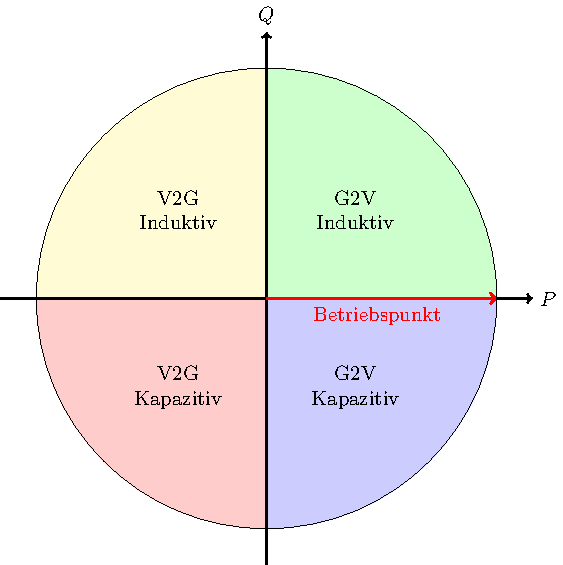
\includegraphics[width=0.7\textwidth]{Bilder/four-quadrant_operation}
    \caption{Mögliche Betriebszustände der Ladetechnik von Elektrofahrzeugen \cite{He2020}}\label{fig:four-quadrant}
\end{figure}

So können Ladevorgänge sowohl blindleistungfrei erfolgen, als auch induktiv oder kapazitiv und werden unter der Bezeichnung \gls{G2V} zusammengefasst.
In \autoref{fig:four-quadrant} entspricht dieser Modus einer positiven Wirkleistung.
Weiterhin können mit bidirektionaler Ladetechnik \glspl{EPKW} ebenfalls entladen werden, um beispielsweise Systemdienstleistungen zu erbringen.
Ein solcher Modus wird allgemein unter der Bezeichnung \gls{V2G} zusammengefasst und kann ebenfalls blindleistungsfrei, induktiv oder kapazitiv erfolgen.
In \autoref{fig:four-quadrant} entspricht dieser Modus einer negativen Wirkleistung. \cite{He2020} 
Innerhalb dieser Arbeit erfolgen Ladevorgänge immer blindleistungsfrei, welches dem Betriebspunkt in \autoref{fig:four-quadrant} entspricht.
Ebenfalls wird der Einsatz von bidirektionaler Ladetechnik nicht untersucht.\medskip

Die einzelnen Ladevorgänge werden anhand ihrer Wirkleistung grob in Normal- und Schnellladevorgänge unterteilt.
Normalladevorgänge finden bei einer Wirkleistung von maximal \SI{50}{\kw} statt, während Schnellladevorgänge bei einer Leistung von \SIrange[range-phrase=~{oder}~]{150}{350}{\kw} stattfinden.
Dabei besitzen die Ladevorgänge pauschal einen Wirkungsgrad von \SI{90}{\percent}.
Eine Übersicht der in dieser Arbeit verwendeten netz- und fahrzeugseitigen Wirkleistungen von Ladepunkten findet sich in \autoref{tab:charging_cap}.
Weiterhin sind die in \autoref{tab:TechPowerCap} zusammengefassten Limitierungen der \glspl{EPKW} zu berücksichtigen.
Unabhängig von der Ladetechnik wird angenommen, dass am Netzverknüpfungspunkt immer einer symmetrische Last anliegt.

{
\renewcommand{\arraystretch}{1.2}% grßerer Zeilenabstand
\sisetup{range-phrase=~bis~}
\begin{table}[H]
	\begin{center}
		\caption{Netz- und fahrzeugseitige Wirkleistung der Ladeinfrastruktur}
		\begin{tabu} to \textwidth {X[0.5] X[1, r] X[1, r]}
			\hline
			\multicolumn{1}{l}{}           		& Netzseitige Wirkleistung & Fahrzeugseitige Wirkleistung \\ \hline
			\multirow[t]{4}{*}{Normalladung} 	& \SI{3.7}{\kw}            & \SI{3.3}{\kw}                \\
										   		& \SI{11.0}{\kw}           & \SI{9.9}{\kw}                \\
										   		& \SI{22.0}{\kw}           & \SI{19.8}{\kw}               \\
										   		& \SI{50.0}{\kw}           & \SI{45.0}{\kw}               \\ \hline
			\multirow[t]{2}{*}{Schnellladung} 	& \SI{150.0}{\kw}          & \SI{135.0}{\kw}              \\
										   		& \SI{350.0}{\kw}          & \SI{315.0}{\kw}              \\ \hline
		\end{tabu}
		\label{tab:charging_cap}
	\end{center}
	\vspace{-3mm}%Put here to reduce too much white space after your table
\end{table}
}


\paragraph{Ladestrategien:}

Der Ladevorgang von \glspl{EPKW} kann durch unterschiedliche äußere Anreize gesteuert werden.
Grundsätzlich lassen sich hierbei marktorientierte und netzdienliche Ladestrategien unterscheiden.


\subparagraph{Marktorientierte Ladestrategien} haben als Fokus die Minimierung der Kosten für den Strombezug. Dies bedeutet konkret, dass die Ladevorgänge durch ein Preissignal am überregionalen Großhandelsmarkt ausgelöst beziehungsweise unterbrochen werden.
Eine solche Ladestrategie kann sowohl positive als auch negative Effekte auf das Stromnetz aufweisen und erfordert einen geeigneten rechtlichen Rahmen.
So führt beispielsweise ein hohes Stromangebot zu niedrigen Großhandelsmarktpreisen, wodurch das beladen der \glspl{EPKW} ausgelöst wird und ein Ausgleich zwischen Angebot und Nachfrage angestrebt wird.
Auf der anderen Seite werden lokale Netzengpässe nicht berücksichtigt und die Gleichzeitigkeit der Ladevorgänge erhöht sich, wodurch sich der lokale Netzausbaubedarf erhöhen kann. \cite{Agora2019} \cite{Dorendorf2019} \cite{Rehtanz2017}


\subparagraph{Netzdienliche Ladestrategien} setzen hingegen auf die Vermeidung von lokalen Engpässen, welche durch eine hohe Nachfrage entstehen können.
Hierbei kann zwischen präventiven und kurativen Maßnahmen unterschieden werden.
Präventive Maßnahmen sollen Verbraucher veranlassen, ihre Ladevorgänge in Zeiten geringer Netzauslastung zu verlegen.
Dies kann zum Beispiel über monetäre Anreize aber auch über Quoten erfolgen.
Bei kurativen Maßnahmen handelt es sich hingegen um ein aktives Eingreifen durch den Netzbetreiber, welcher bei drohenden Netzengpässen in den Ladevorgang eingreift und diesen unterbricht. \cite{Agora2019}

